\documentclass[11pt,a4paper]{article}

\usepackage[utf8]{inputenc}
\usepackage[T1]{fontenc}
\usepackage[italian]{babel}
\usepackage[margin=2cm]{geometry}
\usepackage{graphicx}
\usepackage{booktabs}
\usepackage{amsmath}
\usepackage{listings}
\usepackage{xcolor}
\usepackage{hyperref}
\usepackage{float}
\usepackage{multirow}
\usepackage{caption}
\usepackage{subcaption}

\hypersetup{
    colorlinks=true,
    linkcolor=black,
    urlcolor=blue,
    citecolor=black
}

\title{\vspace{-1.5cm}Progetto di Scalable and Cloud Programming\\}
\author{Marzia De Maina\\
\small Matricola N. 0001194461\\
\small Alma Mater Studiorum - Università di Bologna\\
\small \texttt{marzia.demaina@studio.unibo.it}}
\date{Anno Accademico 2025--2026}

\begin{document}

\maketitle
\vspace{-0.8cm}


\section{Introduzione}
L'obiettivo del progetto è realizzare un'applicazione distribuita in Scala
e Apache Spark che, dato un dataset di eventi sismici, identifichi la coppia
di località in cui i terremoti si verificano nello stesso giorno con la
massima frequenza, elencando le date in cui tale co-occorrenza si è
verificata. L'analisi viene eseguita sul dataset completo (circa 3,4 milioni
di record) tramite cluster Spark gestiti su Google Cloud Dataproc.

\subsection{Pre-processing sui dati}
Il pre-processing sui dati grezzi è avvenuto come segue:
\begin{itemize}
    \item[-] \textbf{Arrotondamento delle coordinate} alla prima cifra
    decimale con \texttt{HALF\_UP} e utilizzo di \\\texttt{java.math.BigDecimal} per evitare le imprecisioni del floating point.
    \item[-] \textbf{Estrazione della sola data} dall'istante temporale, così
    che la finestra di co-occorrenza sia di un giorno.
    \item[-] \textbf{Deduplicazione} delle terne \texttt{(lat, lon, data)}.
\end{itemize}

\section{Approccio implementato}

L'approccio implementato si basa sul paradigma \textit{map-reduce} di
Spark e sfrutta le RDD per controllare in modo esplicito le fasi di
trasformazione e aggregazione.

\subsection{Rappresentazione compatta dei dati}
Per ridurre l'occupazione di memoria e velocizzare lo shuffle, le strutture
dati usate sono volutamente compatte:
\begin{itemize}
    \item[-] ogni cella geografica è rappresentata dalla \texttt{case class}
    \texttt{Cell(latTenths: Int, lonTenths: Int)}, che memorizza la
    coordinata arrotondata come intero moltiplicato per dieci
    (es. $38{,}8 \rightarrow 388$).
    \item[-] ogni data è codificata come \texttt{Int} nel formato
    \texttt{YYYYMMDD} (es. $2024{-}03{-}12 \rightarrow 20240312$).
\end{itemize}

\subsection{Pipeline di elaborazione}

\subsubsection*{Lettura e ripartizionamento}
Il CSV viene letto come DataFrame e immediatamente ripartizionato in
$N$ partizioni (parametro di configurazione). Il ripartizionamento iniziale
è importante per evitare un'asimmetrua dei dati nelle fasi successive: lo shuffle viene
eseguito una sola volta sul dataset intero anziché correggere uno
sbilanciamento già consolidato.

\subsubsection*{Aggregazione per data con deduplicazione locale}
L'RDD viene aggregato per data con
\texttt{aggregateByKey} usando \texttt{HashSet[Cell]} come accumulatore.
Il \textit{combiner locale} deduplica le
celle direttamente all'interno di ciascuna partizione, prima dello shuffle.
Di conseguenza la quantità di dati trasferiti in rete dipende dal numero
di \textit{celle distinte} per giorno e non dal numero totale di eventi.
Le date con una sola cella vengono filtrate (non possono produrre coppie).
L'RDD risultante è messo in cache perché verrà
riutilizzato due volte: prima per il conteggio delle coppie, poi per il recupero
finale delle date.

\subsubsection*{Generazione delle coppie e conteggio}
Per ciascuna data, le celle sono già ordinate canonicamente. Per ogni
coppia $(i,j)$ con $i<j$ viene emessa la tupla
$\big((\texttt{cell}_i, \texttt{cell}_j), 1\big)$. L'uso di un'iterazione
con indici espliciti su un array pre-ordinato evita di dover normalizzare le coppie che sono già in ordine canonico. Le
occorrenze vengono poi sommate con \texttt{reduceByKey(\_ + \_)}: il
combiner locale di \texttt{reduceByKey} aggrega le occorrenze \textit{in
partizione} prima dello shuffle, riducendo il traffico di rete.

\subsubsection*{Selezione e recupero della coppia vincente}
La coppia con il massimo numero di co-occorrenze è ottenuta tramite una
\texttt{reduce} distribuita sull'RDD dei conteggi, senza raccogliere
l'intero RDD sul driver. L'RDD cached al passo~2 viene filtrato per estrarre le sole date in cui
entrambe le celle della coppia vincente compaiono. In questo modo non è
necessario ricostruire da capo l'aggregazione, che rappresenta la parte
più costosa della pipeline.


\subsection{Considerazioni sull'approccio}
Una soluzione alternativa basata su \texttt{groupByKey} per data, seguita
da \texttt{distinct} per la deduplicazione, è stata valutata e scartata:
\texttt{groupByKey} costringe a trasferire tutti gli eventi nello shuffle
senza riduzione locale, e la deduplicazione richiede uno shuffle
aggiuntivo. Sperimentalmente, su cluster con macchine
\texttt{n2-standard-2}, questa variante è risultata persino fallire con
errori di out-of-memory (Container killed, exit code 143) sui worker.
La pipeline basata su \texttt{aggregateByKey} è invece risultata stabile
in tutte le configurazioni testate.

\section{Analisi}

\subsection{Setup sperimentale}
Gli esperimenti sono stati eseguiti sul \textbf{dataset completo}
(\textasciitilde 3{,}4 milioni di record) su cluster Google Cloud Dataproc.
Per valutare l'impatto del tipo di macchina, sono state testate due
configurazioni hardware:
\begin{itemize}
    \item[-] \texttt{n2-standard-4} (4 vCPU, 16~GB RAM) - macchina richiesta
    dalle specifiche del progetto. A causa del limite della quota CPU
    globale dell'account education ($16$ vCPU complessive), è stato
    possibile testare configurazioni con 2 e 3 worker (master + 3 worker
    = $4 + 3 \times 4 = 16$ CPU, al limite della quota); 4 worker
    avrebbero richiesto 20 CPU, oltre il limite.
    \item[-] \texttt{n2-standard-2} (2 vCPU, 8~GB RAM) - usata per
    completare lo studio con 4 worker, dato che con questa macchina il
    cluster a 4 worker richiede solo $2 + 4 \times 2 = 10$ CPU.
\end{itemize}
Sono stati testati i seguenti valori per il numero di partizioni Spark: \texttt{4, 8, 16, 32, 64, 128, 256}.

\subsection{Risultati grezzi}
L'esecuzione dei 35 test totali è stato realizzata attraverso lo script python automatizzato \texttt{benchmark.py}. I risultati di ogni run vengono salvati incrementalmente in un file di log \texttt{benchmark\_log.txt}.
Le Tabelle~\ref{tab:bench_n4}~e~\ref{tab:bench_n2} riportano i tempi di
esecuzione misurati, rispettivamente per \texttt{n2-standard-4} e
\texttt{n2-standard-2}.

\begin{table}[H]
\centering
\caption{Tempi di esecuzione (s) - cluster con \texttt{n2-standard-4}.}
\label{tab:bench_n4}
\begin{tabular}{c ccccccc}
\toprule
\multirow{2}{*}{\textbf{Workers}} & \multicolumn{7}{c}{\textbf{Partizioni}}\\
\cmidrule(lr){2-8}
 & 4 & 8 & 16 & 32 & 64 & 128 & 256 \\
\midrule
2 & 971{,}89 & 657{,}41 & 521{,}98 & 477{,}32 & 434{,}11 & 379{,}22 & \textbf{358{,}74} \\
3 & 981{,}99 & 594{,}39 & 393{,}49 & 344{,}46 & 306{,}04 & 273{,}06 & \textbf{268{,}27} \\
\bottomrule
\end{tabular}
\end{table}

\begin{table}[H]
\centering
\caption{Tempi di esecuzione (s) - cluster con \texttt{n2-standard-2}.}
\label{tab:bench_n2}
\begin{tabular}{c ccccccc}
\toprule
\multirow{2}{*}{\textbf{Workers}} & \multicolumn{7}{c}{\textbf{Partizioni}}\\
\cmidrule(lr){2-8}
 & 4 & 8 & 16 & 32 & 64 & 128 & 256 \\
\midrule
2 & 2662{,}86 & 1321{,}49 & 980{,}96 & 930{,}70 & 860{,}00 & 808{,}87 & \textbf{780{,}90} \\
3 & 1804{,}11 & 1079{,}47 & 661{,}29 & 618{,}87 & 573{,}18 & 567{,}88 & \textbf{563{,}20} \\
4 &  983{,}68 &  860{,}37 & 517{,}71 & 520{,}13 & 474{,}82 & \textbf{444{,}70} & 465{,}59 \\
\bottomrule
\end{tabular}
\end{table}

\begin{figure}[H]
\centering
\begin{subfigure}{0.49\textwidth}
\centering
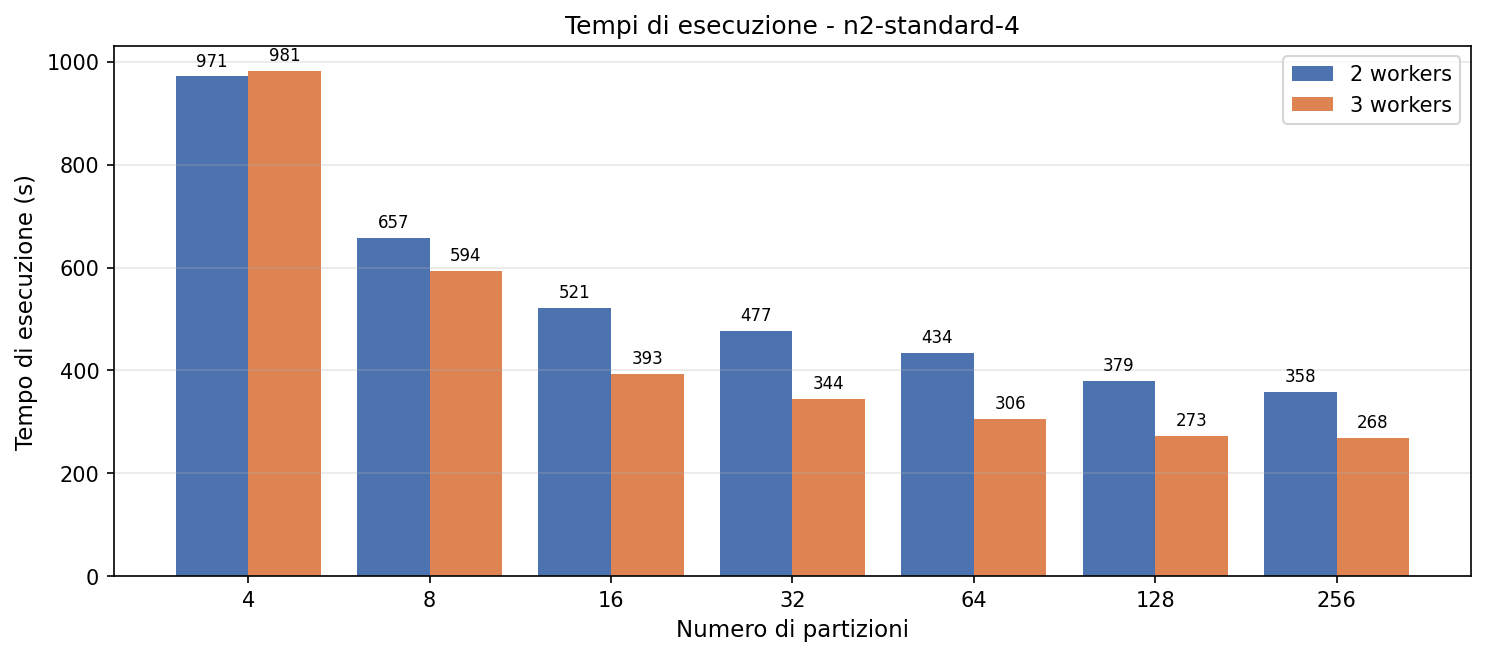
\includegraphics[width=\linewidth]{media/plot_times_n4.png}
\caption{\texttt{n2-standard-4}}
\end{subfigure}\hfill
\begin{subfigure}{0.49\textwidth}
\centering
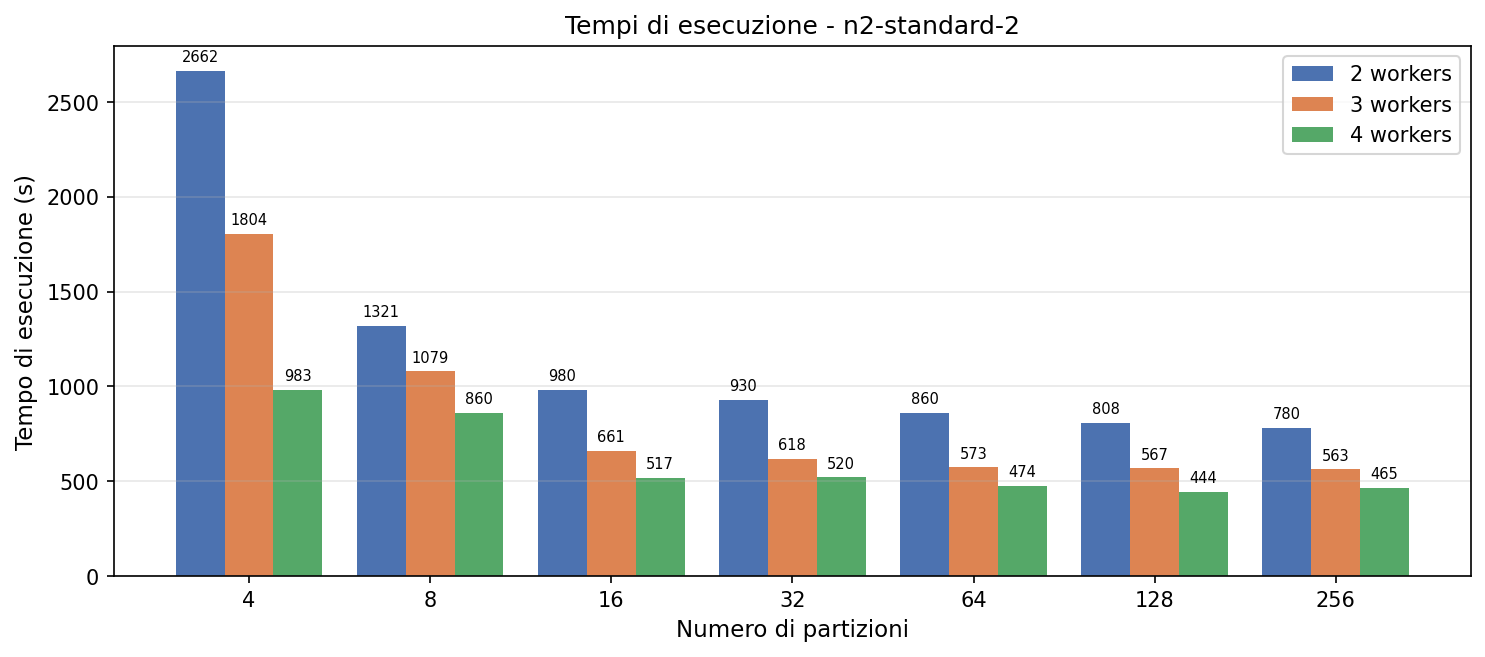
\includegraphics[width=\linewidth]{media/plot_times_n2.png}
\caption{\texttt{n2-standard-2}}
\end{subfigure}
\caption{Tempi di esecuzione per ciascuna combinazione di worker e
partizioni.}
\label{fig:bar}
\end{figure}

\subsection{Impatto del numero di partizioni}

Con 4~partizioni il parallelismo è limitato a 4~task concorrenti. Su un
cluster con 4 worker \texttt{n2-standard-2} sono disponibili $4 \times 2
= 8$ core: solo $4/8 = 50\%$ può essere effettivamente utilizzato.
L'effetto è visibile sia nei cluster \texttt{n2-standard-4} con 3 worker
(tempo praticamente identico a 2 worker: $982$~s vs $972$~s), sia nei
cluster \texttt{n2-standard-2} con 4 worker (tempo $984$~s, addirittura
peggiore di quanto si ottiene aumentando le partizioni). Aumentando il
numero di partizioni a $16$ o più, il tempo si riduce notevolmente perché
i core vengono progressivamente saturati. Al crescere ulteriore del numero di partizioni i miglioramenti diventano
marginali. Per esempio, su \texttt{n2-standard-4} con 3 worker, passando
da $64$ a $256$ partizioni il tempo si riduce solo del $\sim 12\%$
($306 \to 268$~s). In modo simile, su \texttt{n2-standard-2} con 4 worker
il minimo è raggiunto a $128$ partizioni ($445$~s), oltre cui il tempo
addirittura risale leggermente per via dell'overhead di scheduling e dei
costi di shuffle su task molto piccoli.

\begin{figure}[H]
\centering
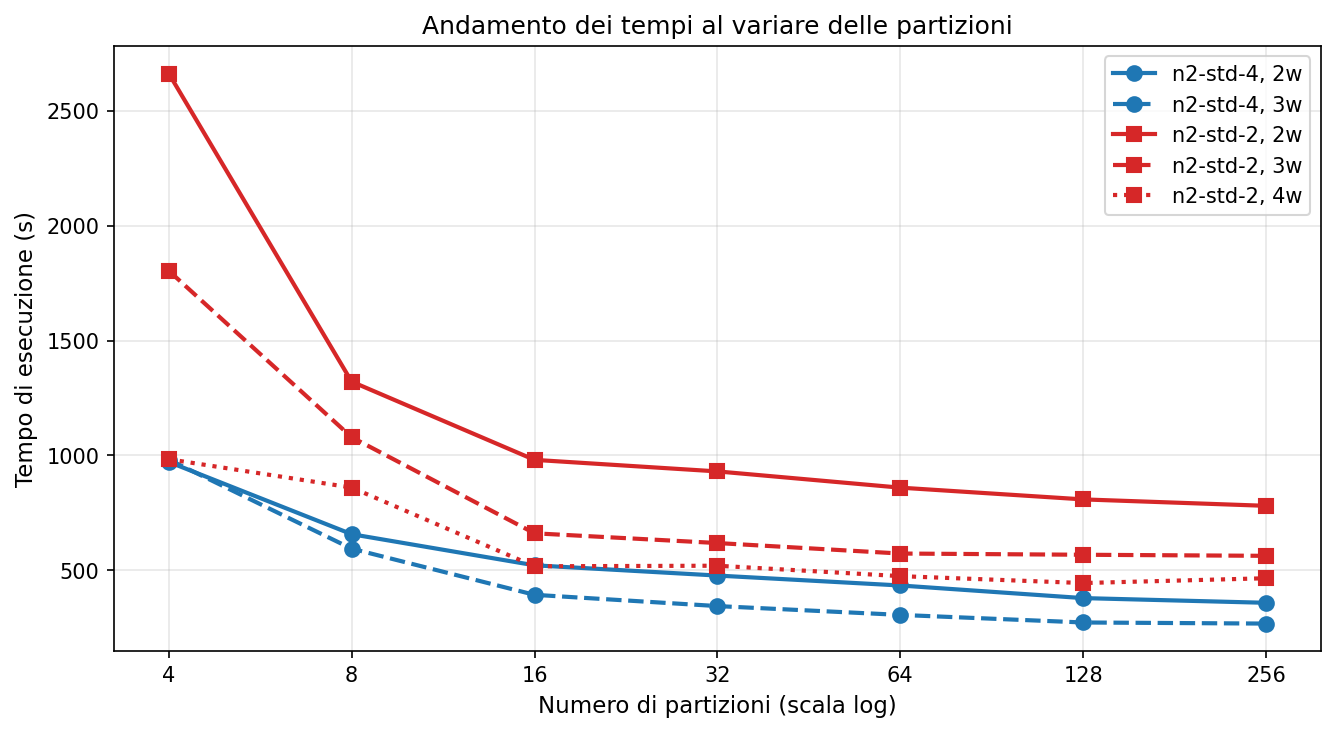
\includegraphics[width=0.9\linewidth]{media/plot_partitions.png}
\caption{Andamento del tempo al crescere del numero di partizioni
(scala logaritmica).}
\label{fig:partitions}
\end{figure}

\subsection{Strong scaling: speedup ed efficienza}
Per ciascun cluster si
considera il tempo di esecuzione ottimale.

\begin{table}[H]
\centering
\caption{Speedup ed efficienza usando i best time per ciascuna
configurazione.}
\label{tab:scaling}
\begin{tabular}{l c c c c}
\toprule
\textbf{Macchina} & \textbf{Workers} & \textbf{Best time (s)} & \textbf{Speedup} & \textbf{Efficienza} \\
\midrule
n2-standard-4 & 2 & 358{,}74 & 1{,}00 & 1{,}000 \\
n2-standard-4 & 3 & 268{,}27 & 1{,}34 & 0{,}891 \\
\midrule
n2-standard-2 & 2 & 780{,}90 & 1{,}00 & 1{,}000 \\
n2-standard-2 & 3 & 563{,}20 & 1{,}39 & 0{,}924 \\
n2-standard-2 & 4 & 444{,}70 & 1{,}76 & 0{,}878 \\
\bottomrule
\end{tabular}
\end{table}

\begin{figure}[H]
\centering
\begin{subfigure}{0.49\textwidth}
\centering
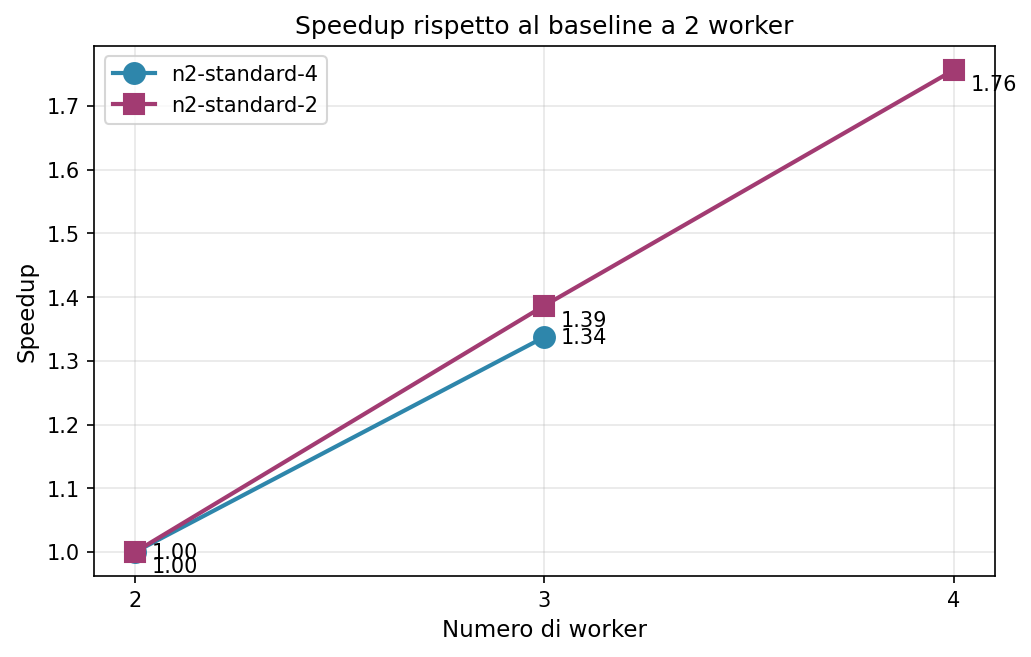
\includegraphics[width=\linewidth]{media/plot_speedup.png}
\caption{Speedup}
\end{subfigure}\hfill
\begin{subfigure}{0.49\textwidth}
\centering
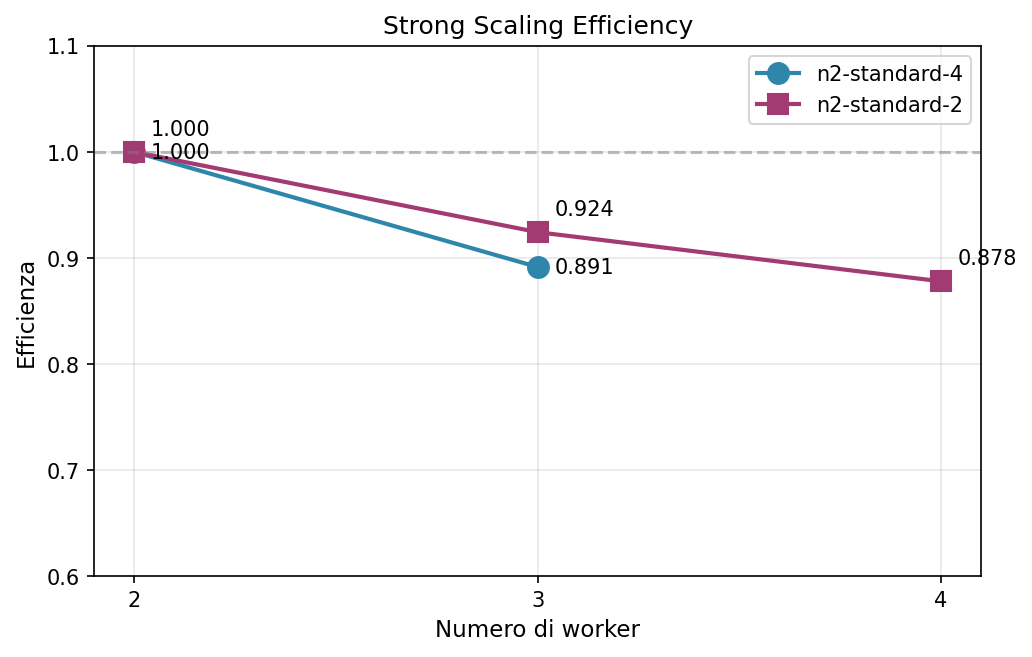
\includegraphics[width=\linewidth]{media/plot_efficiency.png}
\caption{Efficienza}
\end{subfigure}
\caption{Analisi di strong scaling per entrambe le macchine.}
\label{fig:scaling}
\end{figure}
I risultati mostrano una buona scalabilità in entrambe le configurazioni
hardware: sull'\texttt{n2-standard-2} si osserva che l'efficienza
diminuisce leggermente da 3 a 4 worker ($0{,}924 \to 0{,}878$).

\subsection{Parallelizzazione}
Grazie alla legge di Amdahl è possibile stimare la frazione seriale $f$ del workload. Con il range più ampio
disponibile (\texttt{n2-standard-2}, da 2 a 4 worker, quindi $p = 2$ e
$S = 1{,}76$):
\[
f \approx 0{,}14 \quad\Rightarrow\quad
\text{frazione parallelizzabile} \approx 86\%
\]

Questo risultato indica una pipeline ben parallelizzata, con una
componente seriale e di overhead (shuffle, sincronizzazione, scheduling)
attorno al $14\%$.

\section{Conclusioni}
L'approccio basato su \texttt{aggregateByKey} con \texttt{HashSet}
per la deduplicazione locale e \texttt{reduceByKey} per il conteggio
delle coppie permette di eseguire con successo l'analisi sull'intero
dataset entro tempi nell'ordine dei minuti, anche su cluster di
dimensioni modeste. Una variante con \texttt{groupByKey} è stata valutata
e scartata per scarse prestazioni ed errori OOM su macchine piccole.
Il numero di partizioni ha un impatto critico sulle prestazioni:
sotto-partizionare lascia i core inattivi (le configurazioni con 4
partizioni sono circa 3 volte più lente di quelle con 256), mentre
sopra-partizionare introduce overhead non trascurabili.

Il numero di co-occorrenze trovate è 10.014 con la coppia ((38.8, -122.8), (38.8, -122.7)).
\begin{figure}[H]
    \centering
    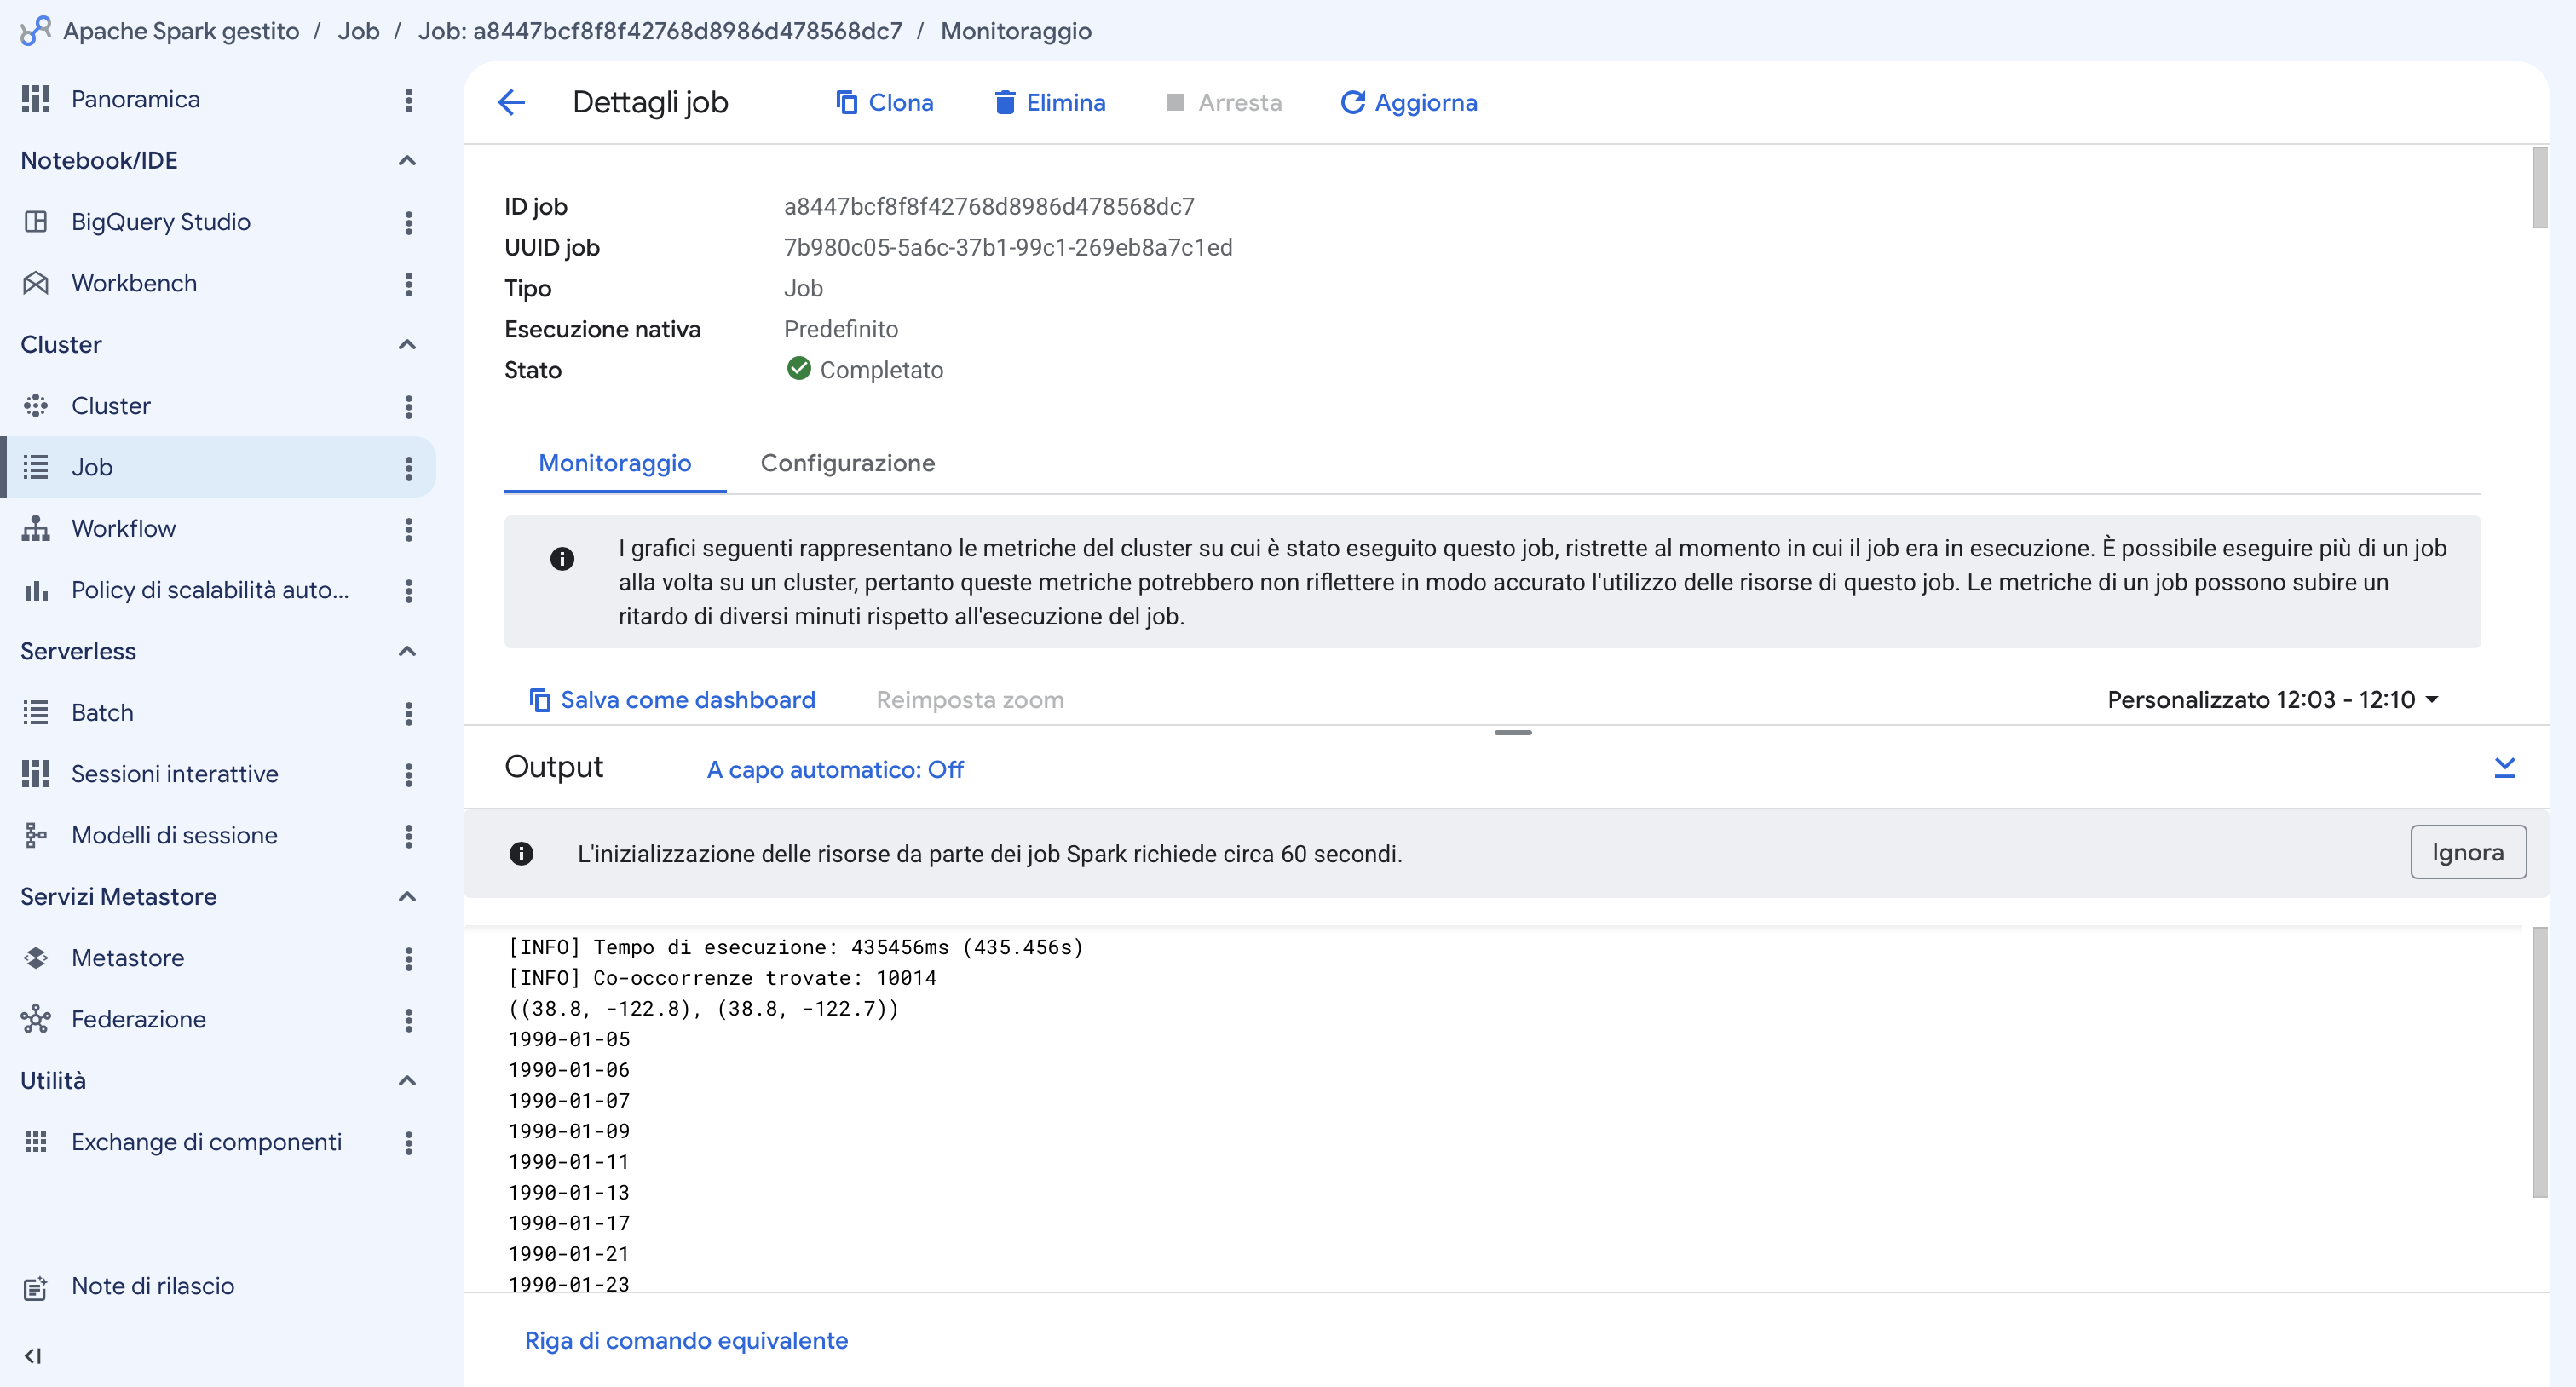
\includegraphics[width=\linewidth]{media/cooccorrenze.png}
    \caption{Esempio di output di co-occorrenze e date.}
    \label{fig:co-occorrenze}
\end{figure}

\section*{Codice Sorgente}
\url{https://github.com/marziademaina/Progetto-di-Scalable-and-Cloud-Programming}.

\end{document}
